\section{Validation and Sensitivity Analysis}

The first validation layer is forecast traceability: Table~\ref{tab:demo-v1-forecast-check} records forecast values and a simple backtest error indicator for each representative material. This prevents the production rule from appearing disconnected from recent demand behavior.

The second validation layer is scenario comparison. Table~\ref{tab:demo-v1-scenario-compare} compares average service level and minimum inventory under the two capacity assumptions. This is a route-specific production check: the paper should show whether stronger capacity meaningfully improves support ability.

\begin{table}[H]
\centering
\caption{Service-level comparison between two capacity scenarios}
\label{tab:demo-v1-scenario-compare}
\begin{tabular}{lrrrr}
\toprule
Material & Service $k_1$ & Service $k_2$ & Min. inv. $k_1$ & Min. inv. $k_2$ \\
\midrule
M1 & 92.85\% & 100.00\% & -9.08 & 7.70 \\
M2 & 94.39\% & 100.00\% & -5.61 & 6.31 \\
M3 & 98.78\% & 100.00\% & -1.14 & 5.77 \\
\bottomrule
\end{tabular}
\end{table}


The table shows a useful stress signal for the demo: under the tighter $k_1$ setting, the average service level drops below the ideal level for M1 and M2, and the minimum inventory becomes negative for all three materials. Under $k_2$, all three representative materials recover to full service with positive inventory buffers. This gives the paper a genuine scenario-comparison story rather than a purely decorative robustness section.

Figure~\ref{fig:demo-v1-scenario} visualizes the same scenario difference. The higher-capacity scenario is never worse on average service level, which makes it a useful reference case for future solver-based improvements.

\begin{figure}[H]
\centering
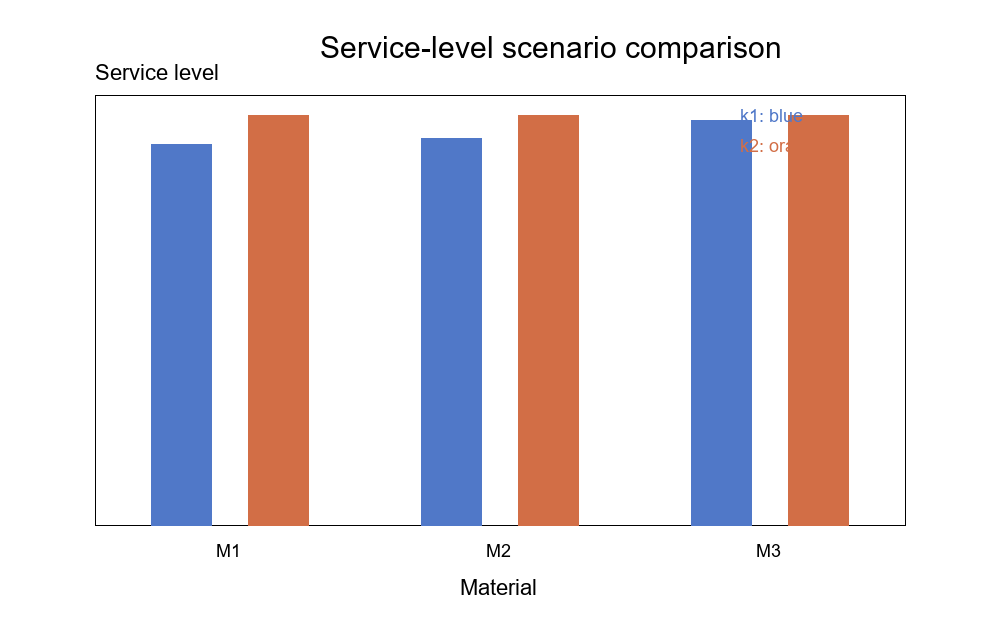
\includegraphics[width=0.85\textwidth]{figures/demo_v1_scenario_compare.png}
\caption{Average service-level comparison between the two capacity scenarios.}
\label{fig:demo-v1-scenario}
\end{figure}

The current v1.0 version is still intentionally conservative. A stronger production-route E paper should add at least three more checks: demand perturbation, coefficient-band sensitivity, and solver comparison against the rolling baseline. The demo writes the route correctly, but it does not pretend to be a final contest-grade optimization study.
